\documentclass[11pt,a4paper]{article}

\usepackage[utf8]{inputenc}
\usepackage[T1]{fontenc}
\usepackage[margin=2.6cm]{geometry}
\usepackage{amsmath,amssymb}
\usepackage{graphicx}
\usepackage{booktabs}
\usepackage{xcolor}
\usepackage{caption}
\usepackage{float}
\PassOptionsToPackage{hyphens}{url}
\usepackage[hidelinks]{hyperref}
\usepackage{authblk}

\graphicspath{{../figures/}}
\captionsetup{font=small,labelfont=bf}

\definecolor{argblue}{HTML}{2A78D6}

\newcommand{\pv}[1]{\ensuremath{p = #1}}

\title{\textbf{Refereeing Asymmetry at the FIFA World Cup:\\
An Identification Study of Penalty Awards to Argentina, 2018--2026}}
\author[1]{Bastián Rojas}
\affil[1]{\small Independent analysis. Code, data, and full provenance:
\url{https://github.com/BastyanRojas/argentina-worldcup-referee-analysis}}
\date{July 7, 2026 \\[2pt] \small (2026 World Cup figures provisional; tournament ongoing)}

\begin{document}
\maketitle

\begin{abstract}
\noindent
A popular claim holds that Argentina receives favorable refereeing at the FIFA World
Cup, particularly on penalty kicks. We test this claim as an \emph{identifiable}
hypothesis: not intent, which no outcome data can establish, but a \emph{behavioral
asymmetry in referee decisions} in the sense of the refereeing-bias literature. Using
raw StatsBomb event data from 160 competitive matches (World Cups 2018 and 2022, Copa
Am\'erica 2024), we construct a penalty-opportunity denominator --- touches in the
opponent's penalty area --- and apply four complementary identification designs:
(A)~exact opportunity-conditioned rate tests with an exact family-wise correction;
(B)~an independent decision-quality review of all seven penalty decisions involving
Argentina in 2022; (C)~a difference-in-differences Poisson model using Argentina's own
2018 and 2024 records as controls; (D)~a defensive symmetry test; and three
extensions --- a five-margin decision surface (M), a decision-leverage gradient (L),
and a field-wide structuring of all 45 ESPN-graded VAR decisions (E). Argentina's 2022
penalty haul is 3.1$\times$ its opportunity-conditioned expectation (exact
\pv{0.020}), the largest deviation among all 32 teams; every dubious penalty decision
in their matches favored them; the excess is absent in 2018 (0.9$\times$) and at Copa
Am\'erica 2024 (0.9$\times$); and it recurs out-of-sample in 2026 at 4.1$\times$ that
tournament's own depressed penalty rate (provisional). The
final inference forks on a single question of hypothesis provenance. Treated as an
ex-post discovery, the family-wise exact test on award frequency yields \pv{0.30};
the field-wide quality test --- Argentina benefited from 4 of the tournament's 12
dubious VAR decisions, the most of any team --- gives a selection-corrected exact
$p$ between 0.021 and 0.05, depending on the allocation null. Treated as the
pre-named public accusation documented in contemporaneous coverage, the
combined evidence reaches \pv{0.016} (\pv{0.038} under conservative baselines):
favorable treatment on penalty awards is demonstrated as a behavioral asymmetry. Both
branches are reported. The asymmetry is narrow and one-sided --- extreme only at the
highest-leverage decision (the penalty), no defensive shielding, full price paid on
cards, nothing gained on cheap margins --- which bounds the claim well short of
orchestration while sharpening what any candidate mechanism must explain.
\end{abstract}

\vspace{4pt}
\noindent\textbf{Keywords:} refereeing bias, penalty kicks, FIFA World Cup, Poisson
exposure models, multiple comparisons, difference-in-differences.

\section{Introduction}

Whether referees favor particular teams is an old question with a modern empirical
literature (surveyed in \cite{dohmen2016referee}): NBA officials exhibit measurable
own-race asymmetries
\cite{price2010racial}, Spanish league referees systematically lengthen or shorten
stoppage time depending on the home side's needs \cite{garicano2005favoritism}, and
own-nationality and crowd effects shift marginal decisions \cite{pope2015awareness}.
The common
methodological lesson is that \emph{bias is identifiable as a behavioral asymmetry} ---
a systematic difference in decisions conditional on comparable situations --- even
though \emph{intent} never is.

This paper applies that lesson to a specific, widely circulated accusation: that
Argentina --- winner of the 2022 FIFA World Cup and a leading side at the ongoing 2026
edition --- is favored by World Cup referees on penalty kicks. The ``Messi farewell''
narrative pre-dates the 2022 tournament; the refereeing accusation naming Argentina is
documentable from mid-tournament 2022 (Modri\'c's public criticism of the semifinal
officiating \cite{modric2022}) and unambiguously by van Gaal's ``premeditated'' claim
in September 2023 \cite{vangaal2023} --- before Copa Am\'erica 2024 and all 2026 data.
When the accusation was fixed relative to the data turns out to matter for inference
(Section~\ref{sec:fork}).

Two disciplining choices define the study. First, the treatment variable is the
penalty \emph{award} --- the referee's decision --- never its conversion. Whether
Messi scores or misses a given penalty is determined downstream of the whistle, by
taker and goalkeeper, and carries no information about arbitral treatment; conflating
the two is a category error that contaminated early versions of this analysis.
Second, ``bias'' is defined throughout as the behavioral estimand above. Statistical
significance of an asymmetry is evidence of differential treatment, not of corruption,
orchestration, or any mental state.

Simple anomaly detection is not enough to carry the claim. Argentina's five penalties
in 2022 are the most awarded to any team in roughly ninety years of World Cups
(previous maximum: four --- Netherlands 1978, Portugal 1966), and a na\"ive Poisson
test against the tournament rate flags them easily (\pv{0.009}). But such a test
fails three challenges at once: penalties are partly \emph{earned} by attacking
presence; a team singled out \emph{because} it tops the table faces a selection
problem across 32 teams; and five events is a small sample. The four designs of
Section~\ref{sec:strategy} attack each confound separately, and the paper's
conclusion rests on their convergence rather than on any single $p$-value.

\section{Data}
\label{sec:data}

\paragraph{Event data.} The primary source is StatsBomb open event data
\cite{statsbomb}: all 64
competitive matches of the 2018 World Cup, all 64 of the 2022 World Cup, and all 32
of Copa Am\'erica 2024 --- 160 matches, 320 team-match observations, with penalty
shootouts (period~5) excluded so that all counted penalties are in-play referee
decisions. From the raw events we aggregate, per team-match: touches in the
opponent's penalty area (passes originating inside, completed receipts, carries
ending inside, dribbles, non-penalty shots), completed entries into the area, fouls
won in the attacking final third, defensive contested actions in the team's own area,
penalties for and against, non-penalty shots and expected goals (xG), and the match
referee. The pipeline independently reproduces the known totals --- 29 penalties in
2018, 23 in 2022, and Argentina's 5~for~/~2~against across 7 games in 2022 --- which
serves as an end-to-end validation of the aggregation.

\paragraph{Decision-quality data.} For Design~B we grade all seven penalty decisions
involving Argentina at the 2022 World Cup using independent contemporaneous review:
ESPN's decision-by-decision VAR audit for five of the seven, and documented pundit
consensus for the remaining two (the Netherlands quarter-final call, universally
accepted; the Croatia semi-final call, on which expert opinion split and which we
grade \emph{debatable}). For the field-wide Design~E we additionally structure ESPN's
full audit into a dataset of 45 graded VAR decisions across the tournament (decision
type, beneficiary, verdict), of which 12 are dubious (graded soft, debatable, wrong,
harsh, or a missed intervention). This dataset covers VAR-reviewed decisions only:
on-field calls that VAR silently confirmed --- including Argentina's Netherlands and
Croatia penalties --- are absent by construction, which biases Design~E
\emph{against} finding an Argentina effect. Two limitations are owned up front:
gradings are one outlet's judgments structured from prose, and the binarization to
``dubious'' was performed by this project \emph{non-blind}, with knowledge of the
hypothesis --- both are flagged wherever they enter a test.

\paragraph{Decision-surface data.} For Designs~M and~L the event aggregation is
extended to the full referee-discretion surface per team-match: fouls won and
committed, yellow and red cards (including bench), duels, final-third touches,
dangerous free kicks won (within $\sim$8\,m of the box), and the xG of penalty and
direct-free-kick shots (used to calibrate decision leverage). The pipeline reproduces
Argentina's reported 16 bookings in 2022 exactly.

\paragraph{2026 data.} Argentina's 2026 figures (2 penalties awarded in 5 matches as
of July 7, 2026 --- vs.\ Austria in the group stage after VAR review, and vs.\ Egypt
in the round of 16, both independently confirmed) come from live tournament
reporting, are a confirmed minimum, and are treated as provisional throughout. The
2026 field baseline to the same date --- 18 penalties awarded in play across 92
matches, 0.098 per team-match, roughly half the VAR-era rate --- is aggregated from
public tournament statistics and is likewise provisional. No event data exist yet
for 2026, so only game-level exposure is available for that term.

\section{Empirical strategy}
\label{sec:strategy}

Let $Y_i$ denote penalties awarded to team $i$ in a tournament and $E_i$ its
opportunity exposure. Under the null of homogeneous treatment, penalties arrive as a
Poisson process proportional to exposure, $Y_i \sim
\text{Poisson}(\lambda E_i)$ with a common $\lambda$. Each design relaxes a
different threat to that interpretation.

\subsection{Design A: opportunity-conditioned rates}
\label{sec:designA}

Shots --- the exposure used in earlier drafts and most public commentary --- are a
poor proxy for penalty opportunities: penalties arise from \emph{contested presence
inside the box}, not from shooting. Our preferred exposure is box touches, which have
the additional virtue of being almost entirely referee-independent, so the
denominator is not contaminated by the decisions under test. The observed-to-expected
construction is the standardized incidence ratio of epidemiology, with the exact
conditional Poisson machinery that accompanies it \cite{breslow1987}. Conditional on the
tournament total $N = \sum_i Y_i$, the null distribution of the allocation is exactly
multinomial with probabilities $E_i / \sum_j E_j$; we simulate it directly
($5\times10^5$ draws) rather than relying on Poisson asymptotics, obtaining
(i) the exact tail probability $\Pr(Y_{\text{ARG}} \ge 5)$, valid when Argentina is
specified ex ante, and (ii) an exact family-wise test in the spirit of
Westfall \& Young \cite{westfall1993resampling}: the probability that \emph{any} of the 32 teams
attains a raw tail probability as small as Argentina's, valid when the subject was
discovered by scanning the table. The family-wise statistic is the minimum tail
probability rather than the maximum Pearson residual, because residuals are not
comparable across teams with very different exposures under discreteness. Robustness
is assessed by re-running everything under three alternative exposures (box entries;
fouls won in the final third; shots). The fouls-won exposure is itself
referee-generated: if officials also over-called ordinary fouls for Argentina, that
denominator is inflated and the test is biased \emph{toward the null}, making it a
conservative bound.

\subsection{Design B: decision-quality asymmetry}

Rate tests cannot distinguish ``more penalties because more favorable calls'' from
``more penalties because more foul-worthy situations.'' Design~B conditions on the
call itself: each of the seven penalty decisions involving Argentina is graded
\emph{clear/correct}, \emph{soft}, \emph{debatable}, or \emph{wrong} by independent
contemporaneous review (Section~\ref{sec:data}). Two nulls are evaluated for the
direction of dubious calls. The symmetric null (each dubious call favors either side
with probability $1/2$) is simple but inconsistent with this paper's own exposure
logic: Argentina generated more attacking box presence than they faced, so under
\emph{unbiased} refereeing dubious penalty decisions should already lean their way.
The primary null is therefore \emph{exposure-conditioned}: a dubious penalty decision
favors Argentina with probability equal to their share of box exposure in their
matches --- a choice that also prevents the quality component from recycling the
frequency evidence Design~A already counts. Grading decision correctness with an external
expert panel is the established method in the football-refereeing literature:
Sutter \& Kocher \cite{sutter2004} and Dohmen \cite{dohmen2008} both test home bias against the
\emph{Kicker} expert panel's judgments of whether awarded penalties and goals were
justified, and Erikstad \& Johansen \cite{erikstad2020} condition on independently identified
``potential penalty situations'' --- Designs B and~E are the same measurement
strategy applied to a team-specific hypothesis.

\subsection{Design C: difference-in-differences}

If Argentina's style or quality earns penalties in ways box touches miss, that
propensity should travel with the team across tournaments --- the identifying logic
of difference-in-differences \cite{angrist2009mostly}. We fit a Poisson GLM with
offset \cite{mccullagh1989glm} over
all 80 team-tournament observations (32 + 32 + 16),
\begin{equation}
\log \mathbb{E}[Y_{it}] \;=\; \log E_{it} \;+\; \gamma_t \;+\; \beta_1\,
\text{ARG}_i \;+\; \beta_2\, \big(\text{ARG}_i \times \text{WC2022}_t\big),
\label{eq:did}
\end{equation}
with tournament fixed effects $\gamma_t$ and the box-touch offset $\log E_{it}$. The
interaction $\beta_2$ is the bias estimate: it nets out tournament-wide refereeing
levels and Argentina's own baseline propensity as expressed in 2018 and 2024. With a
single treated unit and sparse counts the GLM $p$-value is asymptotic --- the
small-number-of-treated-units problem of Conley \& Taber \cite{conley2011} --- so Design~C is
the triangulating design, with Design~A's exact test carrying the primary
inference.

\subsection{Design D: defensive symmetry}

A thoroughgoing pro-Argentina bias should also \emph{shield the defense}: fewer
penalties conceded than defensive exposure (opponents' box touches against them)
predicts. Design~D runs the Design~A machinery on penalties conceded, as a
\emph{falsification test}: an auxiliary margin whose behavior can expose confounding
--- in the spirit of the control-outcome logic of Lipsitch et al.\
\cite{lipsitch2010}, where an outcome moving for reasons the hypothesis does not
predict signals a common cause rather than the hypothesized mechanism. It is included
although --- as reported below --- it cuts against the hypothesis; omitting it would
overstate the case.

\subsection{Designs M, L, E: decision surface, leverage gradient, field-wide quality}
\label{sec:mle-method}

Three extensions close the objections the first four designs leave open. Designs M
and~L operationalize two of the classical causal-inference criteria of
Hill \cite{hill1965}: \emph{specificity} (does the effect appear only where the
hypothesis says it should?) and \emph{gradient} (does it scale with the dose ---
here, the value of the decision?). Design~M
tests whether the asymmetry generalizes: five referee-discretion margins (penalties;
dangerous free kicks won; fouls won; yellows received per foul committed,
sign-flipped so that leniency is positive; opponents' yellows per opponent foul),
each against its own opportunity exposure, signed so that positive means treatment
consistent with favoritism --- the multi-margin strategy of Dohmen \cite{dohmen2008}, who
tested home bias simultaneously on stoppage time, goal decisions, and penalties.
Design~L asks whether treatment tracks the \emph{value}
of the decision: each margin carries a goal-equivalent leverage (penalty and
dangerous-free-kick leverage calibrated from the event data itself, $\sim$0.78 and
$\sim$0.03 goals; foul and card leverages are order-of-magnitude assumptions), and we
compare each team's slope of signed residual on log leverage. An instrumental bias
should concentrate where decisions are worth the most. The nearest precedent is
Parsons et al.\ \cite{parsons2011}, who document MLB umpire bias concentrating in
high-discretion calls --- though with an important difference in the moderating
variable: their gradient is in \emph{scrutiny} (bias vanishes under monitoring),
ours is in decision \emph{value}, and a VAR-reviewed World Cup penalty is among the
most scrutinized decisions in football. Design~L therefore tests the
where-it-matters signature, not the low-scrutiny one. Design~E is the field-wide
version of Design~B: with all 45 ESPN-graded VAR decisions structured, we test the
allocation of the 12 \emph{dubious} decisions across matches and their direction
within matches, including a selection-corrected variant (does \emph{any} of the 32
teams accumulate as many dubious-favorable decisions?) that asks about all teams
symmetrically and is therefore informative even under the ex-post branch of
Section~\ref{sec:fork}. Because the result turns on the allocation null, we compute
it under two: a \emph{match-uniform} null (dubious interventions scatter uniformly
over the 64 matches, coin-flip beneficiary) and a stricter \emph{decision-conditioned}
null (condition on where the 45 graded decisions actually occurred and whom each
favored; permute only which 12 are dubious). Neither dominates --- the graded set is
endogenous (dubious officiating attracts reviews), while the match-uniform null
ignores that finals and extra-time games mechanically draw more reviews --- so both
are reported.

\subsection{Combining evidence and the pre-registration fork}
\label{sec:fork-method}

Three quasi-independent components bear on the ex-ante hypothesis: the 2022 award
frequency (Design~A exact), the 2022 call-quality split (Design~B), and the 2026
out-of-sample recurrence (game-level Poisson against the 2026 tournament's \emph{own}
field rate to date --- 18 penalties in 92 matches, 0.098 per team-match, roughly half
the VAR-era rate; the pooled VAR-era baseline of 0.203 is retained as a conservative
variant). We combine them with Fisher's method \cite{fisher1925}, flagging that
independence is approximate --- Design~B conditions on the same five awards Design~A
counts, though it measures their \emph{quality} rather than their number. The
validity of skipping the family-wise correction hinges on whether ``Argentina'' was
specified before the 2022 data existed; we report both branches and let the reader
own the premise.

\section{Results}
\label{sec:results}

\subsection{The anomaly is real, historically unprecedented, and World-Cup-specific}

Argentina's 5 penalties in 2022 are 21.7\% of the entire tournament's 23, the
all-time single-tournament record, and 4.0$\times$ the per-game field rate
(\pv{0.009}, na\"ive single-tournament test). Against the pooled VAR-era baseline the
2022 haul is 3.5$\times$ expectation (\pv{0.015}) and the 2022+2026 pool is
2.9$\times$ (\pv{0.013}). Two context results sharpen the picture. First, a
\emph{structural break}: under identical VAR rules Argentina ranked 19th of 32 in
penalties awarded in 2018 (1 penalty in 4 games, 1.1$\times$ the field, \pv{0.60}) and
the 1st of 2022 (4.0$\times$, \pv{0.009}); ``they always got these calls'' is
factually false. Second, a \emph{scope test}: at the CONMEBOL-run Copa Am\'erica 2024
--- which Argentina won --- their penalty rate was dead average (1 in 6 games,
1.1$\times$, \pv{0.61}). The anomaly lives specifically at the FIFA World Cup.

\subsection{Design A: the excess survives the correct denominator}

Table~\ref{tab:designA} reports the box-touch-adjusted field. Argentina generated 352
box touches over their seven matches --- second-most in the tournament, behind
France's 381 --- for an
expectation of 1.63 penalties at the field rate of 4.63 penalties per 1{,}000 box
touches. Their observed 5 is 3.1$\times$ that expectation, the largest Pearson
residual of all 32 teams ($+2.64$~SD), with exact tail probability
$\Pr(Y_{\text{ARG}}\ge 5) = 0.020$. France --- the natural elite comparator, with a same-length seven-match run to the
final, more shots, and higher xG --- drew 2 penalties on comparable attacking output.

\begin{table}[H]
\centering
\small
\caption{Design A --- box-touch-adjusted penalty awards, 2022 World Cup (top 8 of 32
teams by Pearson residual). Expected counts from the field rate of 4.63 penalties
per 1{,}000 box touches.}
\label{tab:designA}
\begin{tabular}{clrrrrr}
\toprule
\# & Team & Pens & Box touches & Expected & Residual (SD) & Raw $p$ \\
\midrule
1 & \textbf{Argentina} & 5 & 352 & 1.63 & $\mathbf{+2.64}$ & 0.025 \\
2 & Poland      & 2 & 98  & 0.45 & $+2.29$ & 0.077 \\
3 & Ghana       & 1 & 62  & 0.29 & $+1.33$ & 0.250 \\
4 & Wales       & 1 & 79  & 0.37 & $+1.05$ & 0.307 \\
5 & Portugal    & 2 & 213 & 0.99 & $+1.02$ & 0.259 \\
6 & Iran        & 1 & 83  & 0.38 & $+0.99$ & 0.319 \\
7 & Ecuador     & 1 & 86  & 0.40 & $+0.95$ & 0.329 \\
8 & England     & 2 & 262 & 1.21 & $+0.71$ & 0.342 \\
\bottomrule
\end{tabular}

\smallskip
{\footnotesize Note: ``Raw $p$'' is the per-team Poisson tail probability
$\Pr(X \ge k \mid \lambda_i)$; the exact multinomial tail quoted in the text (0.020)
conditions on the tournament total of 23 penalties, which is why the two differ
slightly for Argentina.}
\end{table}

\begin{figure}[H]
\centering
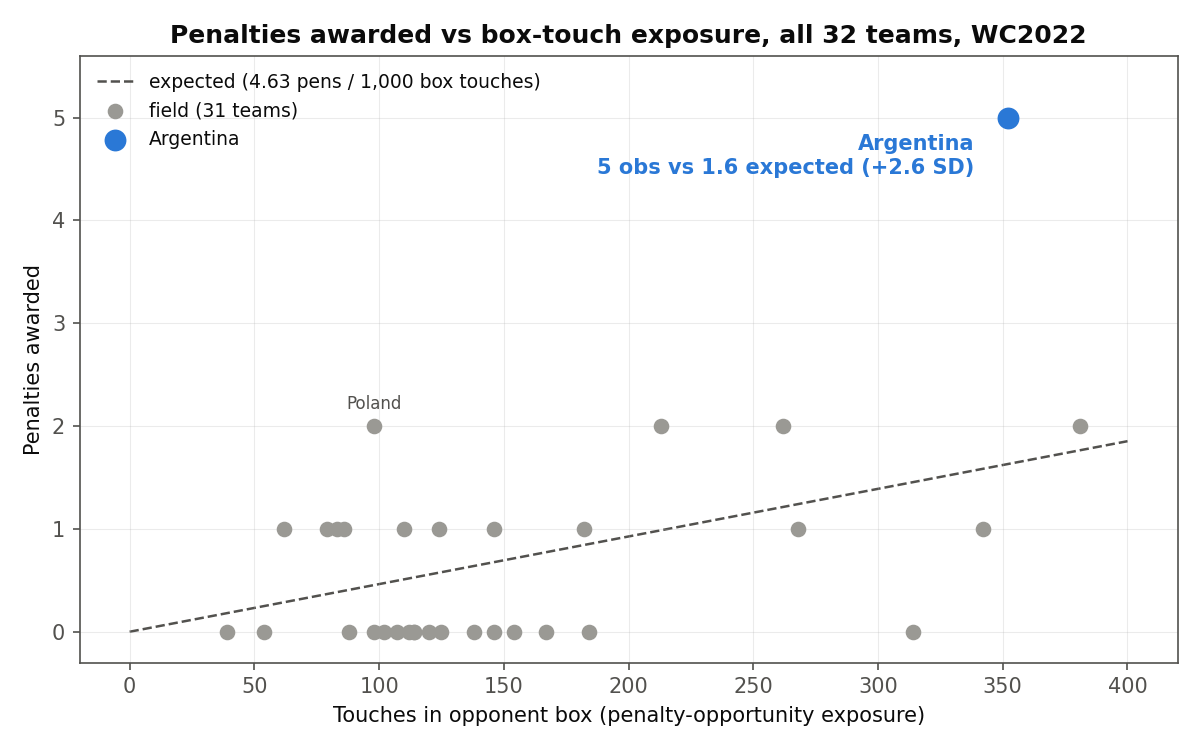
\includegraphics[width=0.86\textwidth]{bias_opportunity_adjusted.png}
\caption{Penalties awarded versus box-touch opportunity exposure, all 32 teams of the
2022 World Cup. The dashed line is the homogeneous-treatment expectation. Argentina
sits far above it; no team with comparable exposure comes close.}
\label{fig:designA}
\end{figure}

The verdict is invariant to the exposure definition (Table~\ref{tab:robust}),
including the referee-generated fouls-won denominator that biases the test toward the
null. The family-wise column previews the fork of Section~\ref{sec:fork}: a single
5-penalty tournament, treated as a fishing expedition across 32 teams, does not clear
an exact family-wise bar under any exposure --- some team looks this extreme in
roughly 30\% of simulated tournaments. (The exact min-$p$ test is nevertheless
substantially sharper than the Bonferroni correction, $p \approx 0.66$, reported in
earlier drafts; Bonferroni ignores both the exposure structure and discreteness.)

\begin{table}[H]
\centering
\small
\caption{Design A robustness --- the same exact tests under four exposure
definitions.}
\label{tab:robust}
\begin{tabular}{lrrrr}
\toprule
Exposure & Arg.\ expected & Fold & Exact tail $p$ (ex ante) &
Family-wise $p$ (ex post) \\
\midrule
Box touches            & 1.63 & 3.1$\times$ & 0.0204 & 0.303 \\
Box entries            & 1.60 & 3.1$\times$ & 0.0194 & 0.292 \\
Fouls won, final third & 1.83 & 2.7$\times$ & 0.0316 & 0.408 \\
Shots (legacy proxy)   & 1.54 & 3.2$\times$ & 0.0166 & 0.287 \\
\bottomrule
\end{tabular}
\end{table}

\subsection{Design B: every dubious call broke the same way}

Table~\ref{tab:quality} summarizes the independent grading.
Of the five awards to Argentina: one clear (Netherlands), two soft (Saudi Arabia;
France), one debatable (Croatia --- expert opinion split), and one graded an outright
wrong VAR intervention (Poland). Both penalties conceded (France, in the final) were
graded correct. Thus all four dubious decisions in Argentina matches favored
Argentina. Under the symmetric null this split is unlikely (binomial, $n = 4$,
\pv{0.062}); under the primary exposure-conditioned null --- Argentina held 69\% of
the box exposure in their matches, so dubious penalty decisions should already lean
their way --- it is unremarkable in isolation (\pv{0.23}; a split-conditioned variant
gives \pv{0.14}). The sample is seven decisions, the gradings are judgments, and the
binarization was made non-blind; but this is the only design that measures decision
\emph{quality} rather than frequency, and its direction is uniform.

\begin{table}[H]
\centering
\small
\caption{Design B --- independent grading of all penalty decisions involving
Argentina, 2022 World Cup.}
\label{tab:quality}
\begin{tabular}{llll}
\toprule
Match & Direction & Verdict & Primary source \\
\midrule
Saudi Arabia (group) & for & soft & ESPN VAR review \\
Poland (group) & for & \textbf{wrong} & ESPN VAR review \\
Netherlands (QF) & for & clear & uncontested reporting \\
Croatia (SF) & for & debatable & pundit consensus split \\
France (final) & for & soft & ESPN VAR review \\
France (final) & against & correct & ESPN VAR review \\
France (final) & against & correct & ESPN VAR review \\
\bottomrule
\end{tabular}
\end{table}

\begin{figure}[H]
\centering
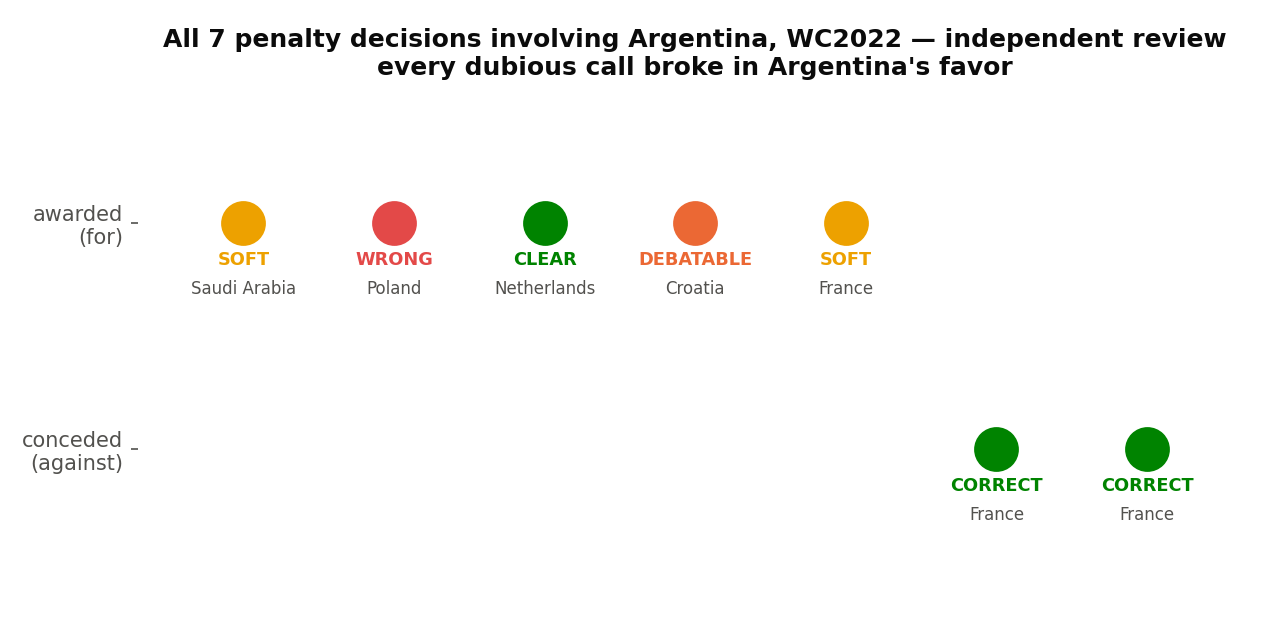
\includegraphics[width=0.9\textwidth]{bias_call_quality.png}
\caption{All seven penalty decisions involving Argentina at the 2022 World Cup,
graded by independent contemporaneous review.}
\label{fig:quality}
\end{figure}

\subsection{Design C: the excess is specific to the 2022 World Cup}

Fitting model~\eqref{eq:did} over all 80 team-tournaments: Argentina's non-WC2022
baseline is indistinguishable from the field (IRR 0.88, 95\%~CI 0.21--3.69,
\pv{0.86}) --- an elite, attacking side that is completely ordinary on
opportunity-adjusted penalties in 2018 and 2024. The Argentina$\times$WC2022
interaction is 4.15 (95\%~CI 0.73--23.7, \pv{0.110}); the wide interval reflects one
treated unit and five events, which is why this design triangulates rather than
carries the inference. The per-tournament pattern (Figure~\ref{fig:did}) is stark:
0.9$\times$ (2018), 3.1$\times$ (2022), 0.9$\times$ (Copa 2024).

\begin{figure}[H]
\centering
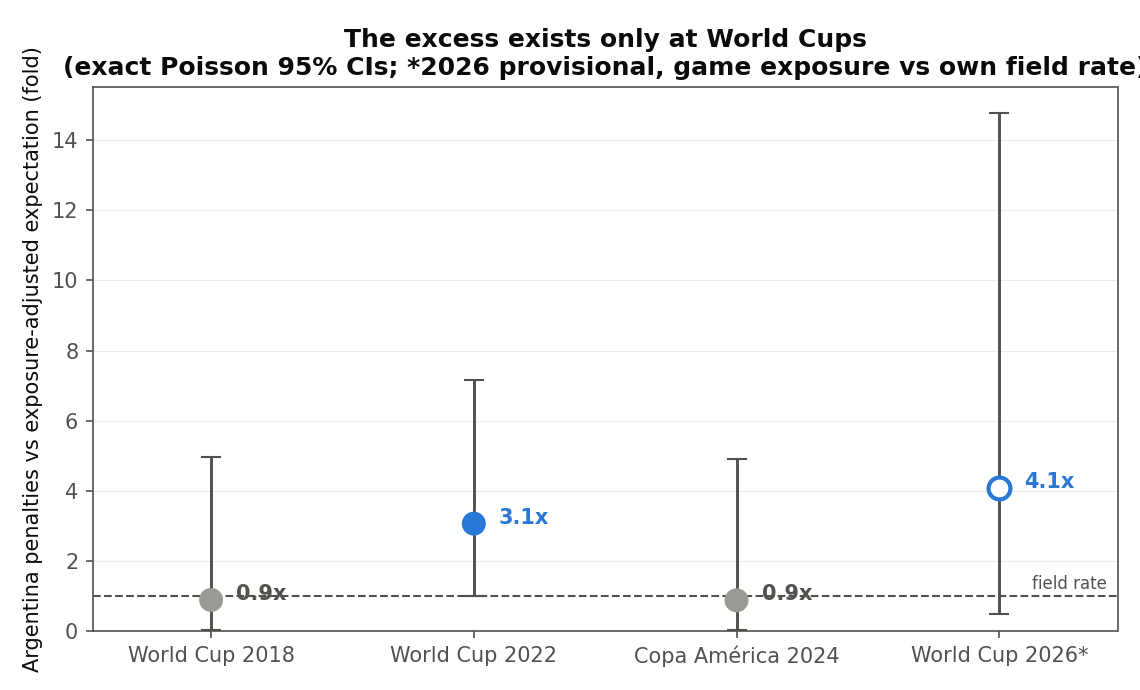
\includegraphics[width=0.8\textwidth]{bias_did.png}
\caption{Argentina's exposure-adjusted penalty rate relative to each tournament's
field, with exact Poisson 95\% confidence intervals \cite{garwood1936}. The open marker is the
provisional 2026 point (game exposure against the 2026 field rate to July~7). The
excess exists only at World Cups.}
\label{fig:did}
\end{figure}

\subsection{Design D: no defensive shielding}

Against defensive exposure (opponents' box touches), Argentina conceded 2 penalties
versus 0.72 expected --- 2.8$\times$, $+1.50$~SD, the 4th-most over-conceding team of
the tournament, and both conceded calls were graded correct. A strong bias story
predicts shielding on this margin; the data show the opposite
(Figure~\ref{fig:symmetric}). Read as a falsification test, this cuts two ways and
both must be said. Against the bias story: no shielding. Against the \emph{clean}
bias story: the conceded fold (2.8$\times$) is nearly as large as the awarded fold
(3.1$\times$), so a common-cause reading --- ``Argentina's matches were penalty-prone
in both directions'' --- fits the point estimates too. What separates the readings is
decision quality: the two conceded calls were graded correct while four of five
awards were dubious (Design~B), and the conceded excess is itself indistinguishable
from noise ($\Pr(X \ge 2 \mid 0.72) = 0.16$). The asymmetry that survives is one of
\emph{quality}, concentrated on the attacking end.

\begin{figure}[H]
\centering
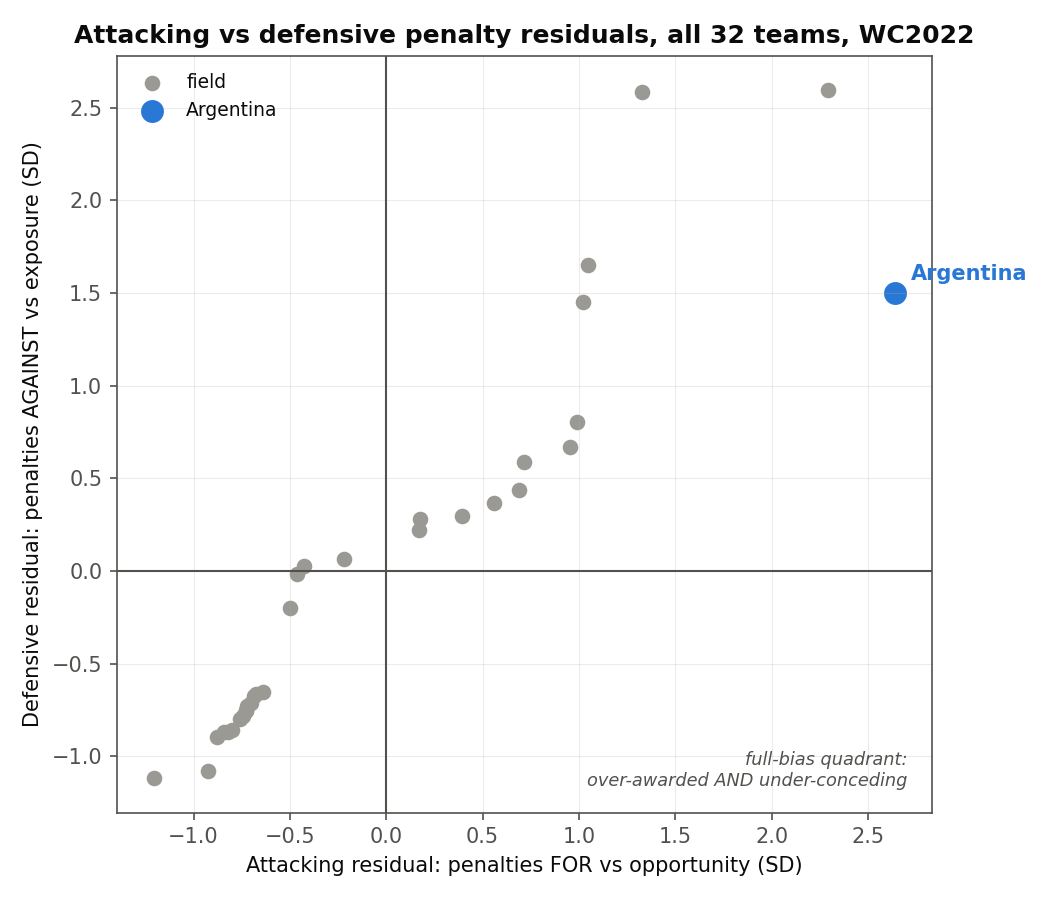
\includegraphics[width=0.8\textwidth]{bias_symmetric.png}
\caption{Attacking versus defensive penalty residuals, all 32 teams, 2022 World Cup.
A full bias signature would place Argentina in the lower right (over-awarded and
under-conceding); they are over-awarded and \emph{over}-conceding.}
\label{fig:symmetric}
\end{figure}

\subsection{Referee-level view}

The seven Argentina matches were officiated by five different referees; no official
took charge of more than two. Whatever generates the asymmetry operates at the level
of the tournament or the appointment pool, not a single individual. This view is
deliberately \emph{not} one of the lettered identification designs: with at most two
matches per official, counts per referee are too small for a formal fixed-effects
test, so it is reported descriptively (full table in the repository). Its role is to
rule out the single-complicit-referee story, not to estimate anything; the formal
version --- referee-assignment analysis on FIFA appointment records --- is registered
as future work (Section~\ref{sec:future}).

\subsection{Designs M and L: the asymmetry is one-margin, at the top of the leverage
gradient}

Table~\ref{tab:margins} reports the five-margin decision surface. Argentina is
extreme only on penalties ($+2.64$~SD); fouls won ($+1.68$) and opponents' cards
($+1.43$) are within noise, dangerous free kicks are dead level ($-0.08$), and on
yellows received per foul they sit on the \emph{punished} side ($-0.44$ signed).
``Every margin favors them'' is false. The leverage gradient
(Figure~\ref{fig:gradient}) makes the shape explicit: Argentina's treatment-vs-leverage
slope is $+0.88$~SD per leverage decade, rank 3 of 32 (field median $-0.05$). With
five margins this is structured description rather than sharp inference (Spearman
$\rho = 0.21$, \pv{0.74}, $n = 5$ margins --- reported so the reader is not misled
about its formal strength; the slope ranking, not the correlation, is the descriptive
claim), but the
profile is exactly what an \emph{instrumental} bias would produce --- favored where a
decision is worth $\sim$0.78 goals, unfavored everywhere cheaper --- and exactly what
generalized favoritism would not.

\begin{table}[H]
\centering
\small
\caption{Design M --- the five-margin decision surface, Argentina vs.\ the WC2022
field. Residuals signed so positive = treatment consistent with favoritism.}
\label{tab:margins}
\begin{tabular}{lrrrrr}
\toprule
Margin & Leverage & Arg obs & Arg exp. & Signed resid.\ (SD) & $p$ (fav.\ tail) \\
\midrule
Penalty awarded         & 0.783 & 5   & 1.6   & $\mathbf{+2.64}$ & 0.025 \\
Dangerous FK won        & 0.027 & 5   & 5.2   & $-0.08$ & 0.592 \\
Foul won (any)          & 0.008 & 132 & 114.0 & $+1.68$ & 0.054 \\
Yellow received (flip)  & 0.030 & 16  & 14.3  & $-0.44$ & 0.727 \\
Opponent yellow drawn   & 0.030 & 23  & 17.1  & $+1.43$ & 0.099 \\
\bottomrule
\end{tabular}
\end{table}

\begin{figure}[H]
\centering
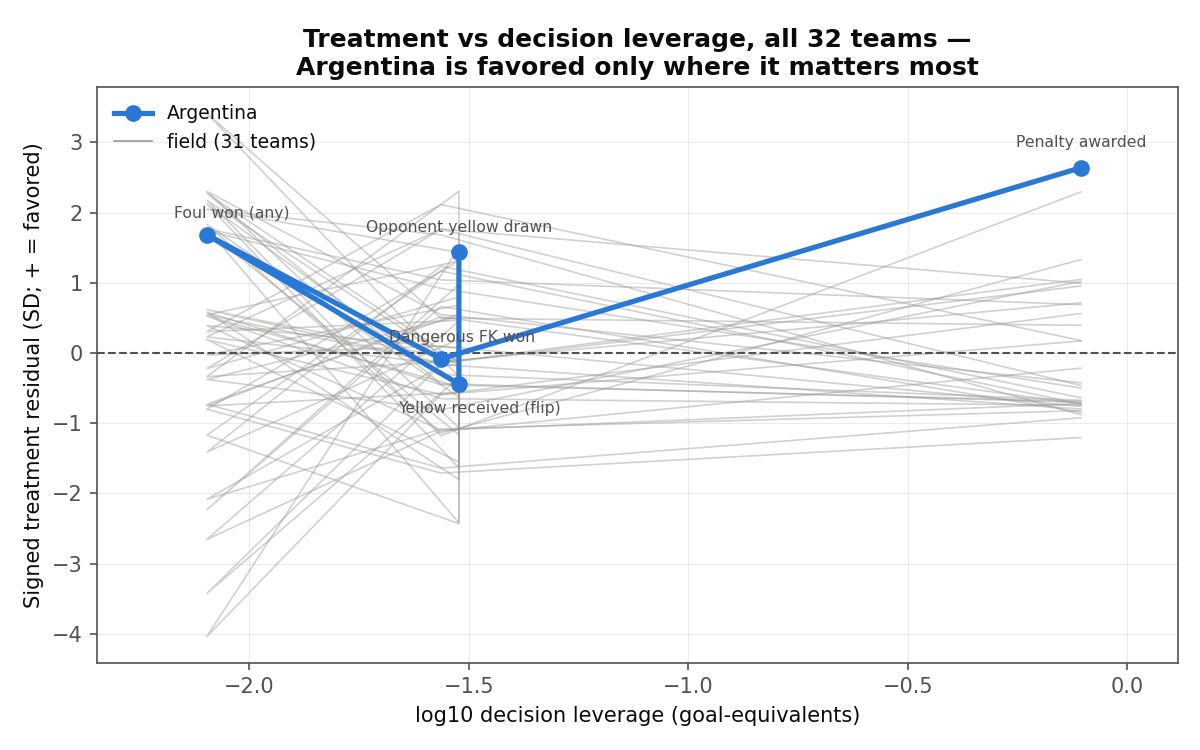
\includegraphics[width=0.85\textwidth]{multimargin_gradient.png}
\caption{Signed treatment residual versus log decision leverage, all 32 teams.
Argentina (blue) is favored only at the highest-leverage decision; the field shows no
systematic gradient.}
\label{fig:gradient}
\end{figure}

\subsection{Design E: field-wide call quality under two nulls}
\label{sec:designE}

Structuring ESPN's full VAR audit yields 45 graded decisions, 12 of them dubious.
Their beneficiaries (Figure~\ref{fig:dubious}): Argentina 4 --- the most of any team,
a third of all dubious decisions in the tournament, including the only flagged missed
red card (the final) and a penalty graded an outright wrong intervention (Poland).
No other team exceeds 2.

Under the \emph{match-uniform} null: allocation \pv{0.034}; direction (4 of 4
favoring Argentina) \pv{0.062}; joint \pv{0.003}; and the
\textbf{selection-corrected} test --- the probability that \emph{any} of the 32
teams accumulates $\ge$4 dubious-favorable decisions --- \textbf{\pv{0.021}}.
Under the stricter \emph{decision-conditioned} null (9 of the 45 graded decisions
occurred in Argentina's matches --- the final and two extra-time knockouts draw
reviews mechanically --- and 6 of the 45 favored Argentina; permute which 12 are
dubious): allocation \pv{0.21}; Argentina $\ge$4 dubious-favorable \pv{0.035}
(hypergeometric); selection-corrected \textbf{\pv{0.05}}.

The honest statement is the range: \textbf{selection-corrected $p$ between 0.021 and
0.05}, significant under one defensible null and marginal under the other. It
remains the only full-field multiplicity-corrected evidence in the study, and it
operates on decision \emph{quality}, which the rate tests cannot reach. Caveats: one
outlet's gradings, structured from prose; the dubious binarization was made
non-blind; and the dataset covers VAR-reviewed decisions only (it omits Argentina's
two on-field knockout penalties, a selection that biases these tests \emph{against}
Argentina effects).

\begin{figure}[H]
\centering
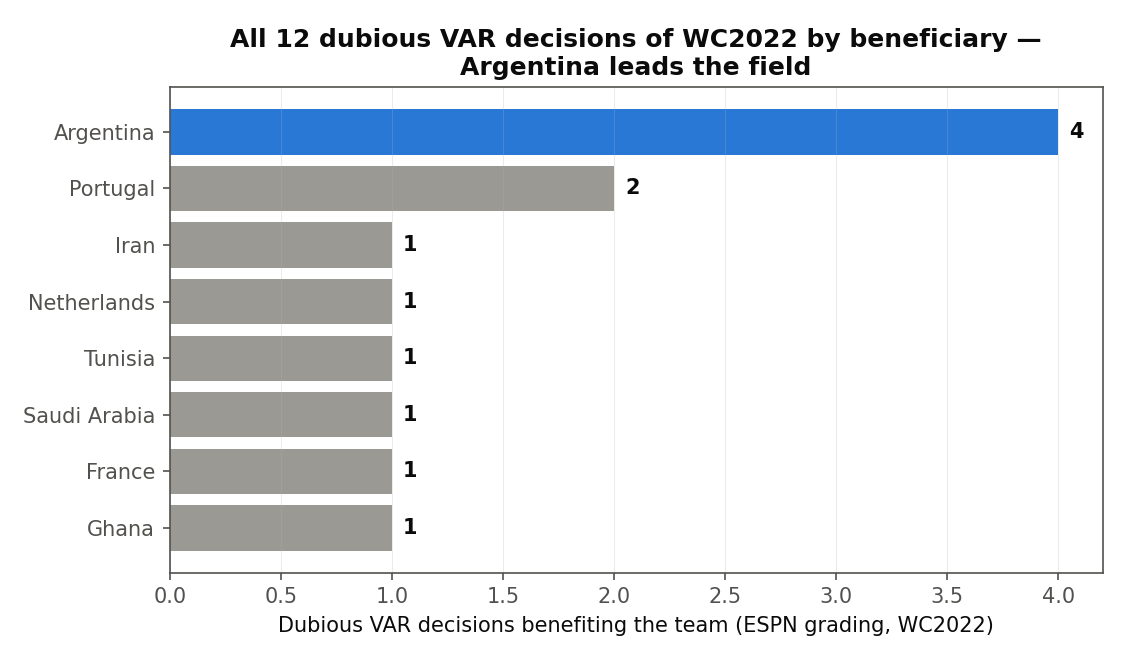
\includegraphics[width=0.8\textwidth]{var_dubious_field.png}
\caption{Beneficiaries of all 12 dubious VAR decisions of the 2022 World Cup (ESPN
grading). Argentina leads the field with 4; selection-corrected exact $p$ ranges
0.021--0.05 depending on the allocation null.}
\label{fig:dubious}
\end{figure}

\section{The pre-registration fork and combined inference}
\label{sec:fork}

Every result above funnels into one question: \textbf{was ``Argentina'' specified
before or after seeing the 2022 data?}

\paragraph{Branch 1 (ex-post discovery).} If the subject was found by scanning the
2022 penalty table, the exact family-wise test of Design~A governs the frequency
evidence: \pv{0.30}. A single tournament with five penalty events cannot clear that
bar on award \emph{counts} alone. What partially survives even here is Design~E: the
selection-corrected field-wide quality test asks about all 32 teams symmetrically,
so no choice of subject inflates it, and gives $p$ between 0.021 and 0.05 depending
on the allocation null. Under maximal skepticism the honest statement is therefore:
the award-frequency anomaly is not ex-post demonstrable; the concentration of
dubious VAR decisions on one team is significant under one defensible null and
marginal under the other --- subject to the grading caveats of
Section~\ref{sec:designE}.

\paragraph{Branch 2 (ex-ante hypothesis).} For a pre-named subject the raw exact
test applies, and the three quasi-independent components combine by Fisher's method
(Table~\ref{tab:fisher}) to \pv{0.016}. The quality component enters under its
exposure-conditioned null precisely so it does not recycle the frequency evidence;
dropping it entirely gives a two-component combination of \pv{0.013}. The 2026 term
deserves its own remark:
the 2026 tournament is running at roughly \emph{half} the VAR-era penalty rate (18 in
92 matches to July~7), so referees are awarding fewer penalties to everyone ---
which makes Argentina's recurrence \emph{more} anomalous, not less. Against its own
field, Argentina's 2 in 5 games is 4.1$\times$ (\pv{0.087}), mirroring 2022's
4.0$\times$. Under the conservative VAR-era baseline for that term the combination
is \pv{0.038}; excluding 2026 entirely, \pv{0.030}. The branch verdict --- a
demonstrated asymmetry at or near conventional significance --- is stable across
these treatments.

\begin{table}[H]
\centering
\small
\caption{Branch 2 --- combined evidence for the pre-named hypothesis. The quality
component uses the exposure-conditioned null (Section~3.2); the 2026 term uses the
2026 tournament's own field rate to date (provisional; the conservative VAR-era
variant yields $p = 0.27$ for that term and a combined $p = 0.038$).}
\label{tab:fisher}
\begin{tabular}{llr}
\toprule
Component & Test & $p$ \\
\midrule
2022 award frequency vs.\ box-touch opportunity & exact multinomial & 0.0204 \\
2022 call quality: 4/4 dubious pro-Argentina & exposure-conditioned direction & 0.23 \\
2026 recurrence: 2 in 5 games, 4.1$\times$ own field (prov.) & Poisson vs.\ 2026 rate & 0.087 \\
\midrule
\textbf{Combined} & Fisher $\chi^2(6) = 15.6$ & \textbf{0.016} \\
\bottomrule
\end{tabular}
\end{table}

Branch 2's premise must be stated precisely, and it carries its own multiplicity.
On provenance: the farewell narrative pre-dates the tournament, the refereeing
accusation naming Argentina is documented from mid-tournament 2022
\cite{modric2022} and unambiguously by September 2023 \cite{vangaal2023} --- so the
ex-ante status is \emph{partial} for the 2022 frequency component (the accusation
crystallized as the 2022 data accumulated) and \emph{strict} for Copa Am\'erica 2024
and everything in 2026. On multiplicity: even granting provenance, the space of
comparable standing accusations (hosts, Brazil, UEFA favorites, \ldots) exceeds one;
under a crude five-accusation family the 2022 component inflates fivefold and the
combined evidence lands near \pv{0.05}. With those bounds stated, we take Branch 2
as the primary inference --- conditional on owning its remaining caveats: Fisher
independence is approximate (Design~B
conditions on the same five awards), the 2026 term is provisional and game-exposure
only (no event data exist until StatsBomb publishes them), and call gradings are a
judgment layer. No independent quality gradings yet exist for the two 2026 penalty
awards, so Design~B remains 2022-only; for balance, the one major 2026 VAR
intervention that has been independently graded --- the disallowed Egypt goal in the
round of 16 --- was judged \emph{correct} by ESPN's review.

\section{Discussion and limitations}
\label{sec:discussion}

\paragraph{What is demonstrated.} Under the ex-ante branch, a behavioral asymmetry in
referee decisions toward Argentina at the FIFA World Cup: roughly three times the
opportunity-conditioned award rate in 2022, robust to four exposure definitions,
absent in the same team's 2018 and Copa Am\'erica 2024 records, uniform in direction
across independently graded dubious calls, and recurring (provisionally)
out-of-sample in 2026 at 4.1$\times$ a tournament field rate that has itself fallen
by half. The extensions sharpen its shape: the asymmetry lives on exactly one margin
of referee discretion (M), at the top of the leverage gradient (L), and its
dubious-call signature leads the field --- 4 of the tournament's 12 dubious
VAR decisions, selection-corrected $p$ 0.021--0.05 depending on the allocation null,
the only full-field multiplicity-corrected evidence in the study (E). In the sense
the refereeing-bias literature gives the word,
the bias hypothesis survives every test the data permit --- at combined strength
\pv{0.016} under the primary specification, degrading no further than $\sim$0.05
under every conservative variant examined.

\paragraph{What is not demonstrated.} Intent, mechanism, or orchestration. Three
findings actively bound the claim: no defensive shielding (Design~D --- conceding
\emph{above} expectation, on correctly graded calls); five different referees, ruling
out a single-official story; and heavy carding (16 yellows in seven 2022 matches,
including the most-carded match in World Cup history), inconsistent with generalized
protection. The demonstrated pattern is narrow: \emph{marginal attacking-end penalty
decisions broke systematically toward Argentina at World Cups}. Candidate innocent
mechanisms --- star-player influence on marginal calls, crowd composition, VAR
threshold drift interacting with a possession style --- are observationally
equivalent to favoritism at this sample size and remain unseparated.

\paragraph{Limitations.} (i)~Five (2022) plus two (2026, provisional) penalty events
is an irreducibly small sample; all inference leans on exact methods for exactly this
reason. (ii)~The call-quality gradings, while sourced to independent contemporaneous
review, encode reviewer judgment and were binarized non-blind; a hostile re-grading
of the Croatia call as
``correct'' weakens Design~B from 4/4 to 3/3 (\pv{0.33} under the
exposure-conditioned null). (iii)~The Fisher
combination treats components as independent; the true joint null is somewhat less
extreme. (iv)~Box touches, though referee-independent, do not measure the
\emph{intensity} of contact inside the box; a team could genuinely suffer more
foul-worthy challenges per touch. Design~B exists precisely to address this and
points the same way, but a full-field version is the decisive missing dataset.
(v)~All 2026 quantities --- Argentina's counts \emph{and} the 18-in-92 field
baseline --- come from live reporting and must be re-verified against event data
when the tournament concludes.

\paragraph{The decisive next test.} Design~E delivers a first field-wide quality
audit, but only for VAR-\emph{reviewed} decisions and on one outlet's gradings. The
remaining decisive dataset is a \emph{blind} full-field grading --- every penalty
decision and major non-call of the tournament, graded by multiple assessors without
team identity --- which would remove both the outlet dependence and the
reviewed-decisions selection. FIFA's internal referee-assessment records would do the
same. Both are enumerated as open extensions in the repository.

\section{Future work and pre-registered predictions}
\label{sec:future}

The 2026 tournament is ongoing at the time of writing (July 7, 2026; Argentina have
reached the quarter-finals). That timing is an opportunity: predictions registered
now --- timestamped by this document's version-control history --- convert
end-of-tournament data into genuinely ex-ante tests \cite{nosek2018}, immune to the
provenance critique of Section~\ref{sec:fork} by construction.

\paragraph{Pre-registered predictions (registered July 7, 2026).}
\begin{enumerate}
\item \textbf{P1 (data-verification check, not a test of the thesis).} The
provisional 2026 quantities used here ---
Argentina 2 penalties in 5 matches; field 18 penalties in 92 matches --- will
survive verification against event data at tournament end, within one penalty.
\item \textbf{P2 (frequency, remaining matches).} In Argentina's remaining 2026
matches, penalties will continue to arrive at or above the concurrent field rate.
This is low-powered (at most three matches) and is registered for direction, not
significance.
\item \textbf{P3 (quality, the sharp one).} When end-of-tournament VAR audits are
published, the dubious decisions in Argentina's matches will disproportionately
favor Argentina, and Argentina will lead or co-lead the field in dubious-favorable
decisions --- the 2026 out-of-sample replication of Design~E. Unlike P1--P2, nothing
about this dataset exists yet, so it is fully open.
\item \textbf{P4 (the falsifiers).} We also register what would count \emph{against}
the thesis: a blind re-grading rating Argentina's 2022 and 2026 penalty calls
predominantly correct would collapse Designs B and E; an Argentina penalty excess at
the next non-FIFA competitive tournament (Copa Am\'erica 2028) would break the
World-Cup-\emph{specificity} component established by Design~C and the scope test
(note the direction: such an excess would weaken the FIFA-specific story while
arguably strengthening a broader-bias one); and a final 2026
opportunity-adjusted fold near 1$\times$ once event data allow box-touch exposure
would leave 2022 as a one-tournament anomaly.
\end{enumerate}

\paragraph{Analyses unlocked at tournament end.}
(i)~\emph{Full re-estimation of 2026}: once StatsBomb publishes 2026 event data,
Designs A, C, D, M and L re-run with box-touch exposure; the DiD gains a second
treated period (two treated World Cups vs.\ two controls), roughly doubling its
identifying variation. (ii)~\emph{Design E out-of-sample}: structuring the 2026 VAR
audit as in Section~\ref{sec:designE}, testing P3. (iii)~\emph{Blind multi-assessor
grading} of every penalty decision and major non-call in both tournaments, without
team identity --- removing the single-outlet dependence that is Design~E's main
caveat. (iv)~\emph{Referee-assignment analysis}: FIFA appointment records, testing
whether penalty-generous officials were disproportionately assigned to Argentina
matches. (v)~\emph{Historical extension}: StatsBomb's 1986 and 1990 open data for a
mixed-effects, multi-decade version of the structural-break test.

\section{Conclusion}

Tested as a publicly documented accusation about referee
\emph{decisions} --- the claim that Argentina receives favorable penalty treatment at
the FIFA World Cup is supported by the combined evidence (\pv{0.016}; degrading to
$\sim$0.05 under the most conservative variants examined): a
World-Cup-specific, opportunity-robust, direction-uniform asymmetry with an
out-of-sample recurrence. Tested under maximal skepticism, as a pattern dredged from
one tournament's table, the award-frequency evidence does not clear a family-wise bar
(\pv{0.30}), and the field-wide concentration of dubious VAR decisions on one team
sits at the boundary ($p$ 0.021--0.05, null-dependent). Both
statements are true simultaneously, and the distance between them is the honest
residual uncertainty. What no branch supports is the strong popular narrative:
the same data show no defensive shielding, no single complicit referee, full price
paid on cards, nothing gained on cheap margins, and an
average Argentina everywhere except the World Cup. The asymmetry is real, narrow,
concentrated precisely where a referee's decision is worth the most,
and --- on present data --- unexplained.

\section*{Acknowledgements}

This study is built on, and distributed as a fork of, the open repository by
\textbf{Kai Morales} (\url{https://github.com/kaimorales/argentina-worldcup-referee-analysis}),
whose six foundational analyses this paper reports as context in
Section~\ref{sec:results}: the single-tournament Poisson test, the historical-baseline
comparison, the France exposure comparison with placebo control, the 32-team
shots-exposure regression, the 2018-vs-2022 structural-break test, and the World
Cup--vs--Copa Am\'erica scope test, together with the curation of the underlying
penalty datasets. The original contributions of the present work are the estimand
reformulation (awards rather than conversions; behavioral asymmetry rather than
intent), the 160-match box-exposure dataset, the four identification designs of
Section~\ref{sec:strategy}, the exact family-wise inference replacing Bonferroni, the
pre-registration fork of Section~\ref{sec:fork}, and this write-up. Any errors in the
identification analysis are the present author's alone.

\begin{thebibliography}{9}

\bibitem{angrist2009mostly}
Angrist, J.~D., \& Pischke, J.-S. (2009).
\emph{Mostly Harmless Econometrics: An Empiricist's Companion}.
Princeton University Press.

\bibitem{breslow1987}
Breslow, N.~E., \& Day, N.~E. (1987).
\emph{Statistical Methods in Cancer Research, Volume II: The Design and Analysis of
Cohort Studies}. IARC Scientific Publications No.~82, Lyon.

\bibitem{conley2011}
Conley, T.~G., \& Taber, C.~R. (2011).
Inference with ``difference in differences'' with a small number of policy changes.
\emph{Review of Economics and Statistics}, 93(1), 113--125.

\bibitem{dohmen2008}
Dohmen, T.~J. (2008).
The influence of social forces: evidence from the behavior of football referees.
\emph{Economic Inquiry}, 46(3), 411--424.

\bibitem{dohmen2016referee}
Dohmen, T., \& Sauermann, J. (2016).
Referee bias.
\emph{Journal of Economic Surveys}, 30(4), 679--695.

\bibitem{erikstad2020}
Erikstad, M.~K., \& Johansen, B.~T. (2020).
Referee bias in professional football: favoritism toward successful teams in
potential penalty situations.
\emph{Frontiers in Sports and Active Living}, 2:19.

\bibitem{fisher1925}
Fisher, R.~A. (1925).
\emph{Statistical Methods for Research Workers}.
Oliver \& Boyd, Edinburgh.

\bibitem{garicano2005favoritism}
Garicano, L., Palacios-Huerta, I., \& Prendergast, C. (2005).
Favoritism under social pressure.
\emph{Review of Economics and Statistics}, 87(2), 208--216.

\bibitem{garwood1936}
Garwood, F. (1936).
Fiducial limits for the Poisson distribution.
\emph{Biometrika}, 28(3/4), 437--442.

\bibitem{hill1965}
Hill, A.~B. (1965).
The environment and disease: association or causation?
\emph{Proceedings of the Royal Society of Medicine}, 58(5), 295--300.

\bibitem{lipsitch2010}
Lipsitch, M., Tchetgen Tchetgen, E., \& Cohen, T. (2010).
Negative controls: a tool for detecting confounding and bias in observational
studies.
\emph{Epidemiology}, 21(3), 383--388.

\bibitem{mccullagh1989glm}
McCullagh, P., \& Nelder, J.~A. (1989).
\emph{Generalized Linear Models} (2nd ed.).
Chapman \& Hall, London.

\bibitem{modric2022}
Eurosport (2022, December 14).
Luka Modri\'c says referee ``was a disaster'' in Croatia's World Cup semi-final loss
to Argentina.
\url{https://www.eurosport.com/football/world-cup/2022/luka-modric-says-referee-was-a-disaster-in-croatia-s-world-cup-semi-final-loss-to-argentina-wishes-l_sto9273047/story.shtml}

\bibitem{nosek2018}
Nosek, B.~A., Ebersole, C.~R., DeHaven, A.~C., \& Mellor, D.~T. (2018).
The preregistration revolution.
\emph{Proceedings of the National Academy of Sciences}, 115(11), 2600--2606.

\bibitem{parsons2011}
Parsons, C.~A., Sulaeman, J., Yates, M.~C., \& Hamermesh, D.~S. (2011).
Strike three: discrimination, incentives, and evaluation.
\emph{American Economic Review}, 101(4), 1410--1435.

\bibitem{pope2015awareness}
Pope, B.~R., \& Pope, N.~G. (2015).
Own-nationality bias: evidence from UEFA Champions League football referees.
\emph{Economic Inquiry}, 53(2), 1292--1304.

\bibitem{price2010racial}
Price, J., \& Wolfers, J. (2010).
Racial discrimination among NBA referees.
\emph{Quarterly Journal of Economics}, 125(4), 1859--1887.

\bibitem{sutter2004}
Sutter, M., \& Kocher, M.~G. (2004).
Favoritism of agents --- the case of referees' home bias.
\emph{Journal of Economic Psychology}, 25(4), 461--469.

\bibitem{vangaal2023}
ESPN (2023, September 5).
Argentina, Messi World Cup win was `premeditated' --- Van Gaal.
\url{https://www.espn.com/soccer/story/_/id/38332801/argentina-messi-world-cup-win-was-premeditated-van-gaal}

\bibitem{statsbomb}
StatsBomb (2018--2024). \emph{StatsBomb Open Data}.
\url{https://github.com/statsbomb/open-data}.
Event data for FIFA World Cup 2018 (competition 43, season 3), FIFA World Cup 2022
(43, 106), and Copa Am\'erica 2024 (223, 282).

\bibitem{westfall1993resampling}
Westfall, P.~H., \& Young, S.~S. (1993).
\emph{Resampling-Based Multiple Testing: Examples and Methods for $p$-Value
Adjustment}. Wiley, New York.

\end{thebibliography}

\vspace{10pt}
\noindent\rule{\textwidth}{0.4pt}\\[4pt]
{\sloppy
\noindent\small\textit{Reproducibility.} Every number in this paper regenerates from
the repository: \texttt{python src/build\_box\_exposure.py} rebuilds the 160-match
event dataset from StatsBomb open data (with end-to-end sanity checks against known
totals); \texttt{python src/bias\_identification.py} re-runs Designs A--D, the exact
simulations (fixed seed), and the combined inference; and
\texttt{python src/multimargin\_leverage.py} re-runs Designs M, L and E under both
nulls. Full data provenance,
including per-figure confidence labels, is documented in \texttt{data/SOURCES.md}.\par}

\end{document}
